\chapter[SCP-179 星海瞭望]{
    SCP-179 Sauelsuesor\\
    SCP-179 星海瞭望
}

\label{chap:SCP-179}

\bb{项目编号:}SCP-179

\bb{项目等级:}\dd{Safe} Thaumiel

\bb{特殊收容措施:}SCP-179当前处在任何已知同行组织和基金会自身的控制范围外。收容尝试将集中于3级\ii{忽略型}掩盖措施的实行,并对一切针对水星轨道内空间、穿越该区域轨道进行探索、研究的太空任务进行干涉和扰乱。

\bb{描述:}SCP-179是一处于外太空中的人形实体。该实体停留于距太阳光圈南极约40000km的位置、即太阳的旋转中轴上,但并不会绕太阳旋转;对SCP-179最近的记录显示它似乎是在绕银河中心旋转。

长达43年连续的观测确认SCP-179的外貌为一20\~{}40岁之间、人种未知的人类女性。该实体的身体表面被一层不光滑的黑色材料包裹。实体的头发超过34km长且一直被太阳风吹动,似乎也是由该种黑色材料构成。不同于其身体,SCP-179的头发会反射着多种太阳光——基金会天体物理学家正是通过该现象于1940年确认了实体的存在。实体身体的中轴上分布有多个标记和符号。从其亮度来判断,这些标记可能有着金属结构并且是金色的。

数个此类标记被发现是中世纪炼金术中常用于表示太阳及太阳系内6颗中央行星的专用象征。依次包括:

\begin{itemize}
\item 表示黄金\slash 太阳的符号位于项目前额、发际线右下方。
\item 表示水银\slash 水星的符号位于项目鼻部并覆盖到嘴唇。
\item 表示铜\slash 金星的符号位于锁骨中段之间。
\item {[}数据删除– 自动审查SC4级– 发现非正常认知危害]形状在解剖学上与人类心脏一致,位于项目胸口大致为同年龄、身材女性人类心脏所在区域的位置。
\item 代表铁\slash 火星的符号位于项目腹部区域上端。
\item 代表锡\slash 土星的符号位于项目腹部区域下端。
\item 最后一个符号部分位于骨盆区域,但由于该位置身体结构的特殊性,对该符号的观察有些困难。不过推测这一代表铅\slash 木星的符号还有部分藏在会阴区域。
\end{itemize}

SCP-179大部分时候都是腹部一侧朝向地球,但偶尔也有机会观察到其背面。{[}数据删除]

{[}更多资料依照行政警ES-026要求删除]

\begin{whiteboxbb}[colframe=textred, parbox=false]
    
\cl{
\fcolorbox{textred}{white}{\makebox[0.8\linewidth]{\g{\tred{\bb{行政警告ES-026}}}}}
}

\begin{minipage}{\textwidth}
\begin{minipage}{0.8\textwidth}
自██\slash ██\slash ████起,SCP-179重分级为Thaumiel。所有权限低于4\slash 179级的相关人员将在SCP-179现任首席研究员的指导下被提高权限或调走以符合该分级要求,具体情况视该人员与对项目的持续观察和掩盖工作实施的相关度而定。所有被调配人员将接受博学者-08记忆编辑疗法或D级记忆删除(给予较高剂量,效力最高影响向前追溯十年内的生活经历),具体情况视其之前在SCP-179上工作的时间长短而定。\\

SCP-179的存在将列入\ii{轨道误报型标准无害情报障碍}类别。依照\ii{忽略}协议4号(第4.5、4.6与4.7条)固定,大部分与SCP-179相关的文件已被分级为4级(最高机密)。任何关于SCP-179的更多信息已被分级为5级(Thaumiel),仅对获得5\slash 179授权的人员开放。
\end{minipage} %
\hfill %
\begin{minipage}{0.15\textwidth}
\centering

\uu{归档警告}


\includegraphics[max width=0.9\linewidth]{images/SCP-179.png}

\uu{限5/179权限}
\end{minipage}
\end{minipage}

\bb{敬告:}对SCP-179研究材料的未授权访问将被视作一次3-B型违规行为(无正当全球权限下的未授权数据管理),惩罚将是强制接受记忆删除治疗并重新调配和\slash 或降级。
\end{whiteboxbb}

\tred{++ 警告!未授权人员将暴露于模因防御触媒中}

\tred{-- 启动模因防御—完形磨石启动}

\begin{figure}[H]
    \centering
    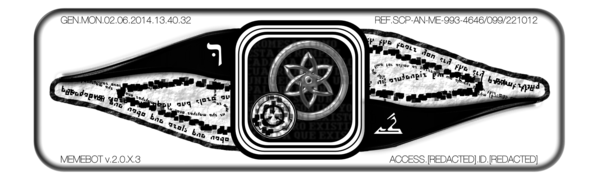
\includegraphics[width=0.8\linewidth]{images/SCP-179-2.png}
\end{figure}

SCP-179对电磁波频谱内的所有辐射均十分敏感,具有智能,并能通过多种异常方式进行交流,包括但不限于对无线电与镭射通信进行干涉。迄今SCP-179仅与基金会人员进行过一次交流,此次交流中SCP-179使用的是流利的法语。然而此次交流并未能清楚获知SCP-179对基金会有何目的,也未知及其自身有何任务;当前所有的努力均集中于防止其他任何已知同行组织与SCP-179发生交流。已经启动信息误报编造操作和其他干预手段。

SCP-179被记录到的行动均与外太空威胁有关,均是针对可能与地球发生碰撞或轨道交叉的异常\slash 非异常天体。当前可以确认若这些威胁天体成功抵达地球,其后果足以CK级重构事件并对人类社会和地球生命在多个方面造成严重打击。而若这些天体与地球的碰撞或轨道交叉未能得到基金会的恰当处置和收容,其后果将有可能是XK级世界末日情景。

SCP-179时常会对单个或集群的此类天体进行定位,之后使用一只手臂指向该天体;若有多个天体同时出现,项目随需要会生出额外的形似手臂的肢体。观测资料显示SCP-179会对每一被定位的天体做出不同的动作——如举起不同的手指或以难以辨认的方式和频率挥动手臂—,这些动作是否包含了什么特殊含义当前仍然未知。

SCP-179的侦测范围极限迄今没有查明。SCP-179已被确认能够侦查到来自海王星轨道外区域以外的潜在威胁天体,这些天体中有部分此前已被其他观察或探索系统(大部分是在基金会控制下)所确认,甚至在至少三个不同的案例中可以由地球裸眼观察确认,但是这些天体并没有在被发现时就立即被确认为威胁。推测SCP-179可能只会针对处在海王星轨道内区域外观测者可见的活跃威胁天体进行侦测和反应,并能无失误地确认其是否具有威胁。所有处于海王星轨道内区域的对地威胁天体都被SCP-179无一遗漏地侦测到,且时常是在基金会已知观测点均未察觉其存在的情况下先行完成。

也因此SCP-179和所有负责对其进行监控的人员、轨道设备设施成为了基金会最可靠的早期预警系统,它能准确地侦测、并在一定情况下阻止可见宇宙内的潜在地外侵入。SCP-179能准确探明哪些天体对地球、人类和地球生物圈具有威胁的特性使得其成为基金会“复合轨道早期预警系统”(COEWS)计划中的关键部分。当前计划还涉及到了SCP-███、SCP-████、SCP-██-████和SCP-████、XCPOA-003到-042\footnote{实验用基金会轨道资产(XCPOA)。}、Site-34、Site-103、Site-98、Area-08、Site-██、Site-███-█、█、█以及Command Site-██,此外数名潜伏进与外太空探索有关的机构、国际组织内部的人员也参与到了计划中。所有通过SCP-179获得或与之相关的数据将被标为COEWS-179,这些数据将成为为基金会各部门使用的高优先级信息。

\bb{附录SCP-179-01:值得注意的SCP-179活动。}

\begin{itemize}
\item \bb{<13\slash 12\slash 1940>} 首次记录到SCP-179活动。实体两手交叉,举手指出了一个此前未被发现的对地威胁天体。在坠入地球后该物体在{[}数据删除]的城市内产生了大量异常粘液,导致了1003人死亡并伴有与{[}依照先前删除已编辑]相关的异常现象。遗留下的核心物体已被分类为SCP-███。SCP-179此后回到了原始姿势。
\item \bb{<22\slash 09\slash 1942>} 第六次记录到SCP-179活动。实体举起手臂指向{[}已编辑],正朝地球撞来。该物体于04\slash 10\slash 1942坠落在新西兰奥克兰附近。该物体在着陆后分裂成数个机械仪器。{[}数据删除]最后产生出了具有较小人员致命性的次生实体。在基金会技工妥当收容该物体后,它被分类为{[}已编辑]并自动消灭了大部分次生实体,SCP-179回到原始姿势。机动特遣队{[}已编辑,所有关于相关资产的数据已从档案中删除]被派往现场并消灭了所有剩余次生实体。
\item \bb{<██\slash ██\slash 19██>} 第十八次记录到SCP-179活动。实体举起右手指向{[}数据删除]。直到此时为止,实体仍然一直保持用一只主要的手臂(会依其需要交替使用不同手臂)指向该方向。
\item \bb{<01\slash 03\slash 1949>} 第23次记录到个体活动。实体举起手臂指向一颗正在撞向地球的艾莫级小行星。基金会使用多个SCP物品联合制作了一台远程控制的星际飞船作为重力拖绳对其进行拦截;该行动于03\slash 05\slash 1951宣告成功;这之后SCP-179回到原始姿势。\ii{\bb{附注:}观察设备发现实体做出了一个类似点头的动作。重分级为Euclid的申请被上交但未被批准。}
\item \bb{<13\slash 12\slash 1998>} 第403次记录到SCP-179活动。实体不再注视地球而是将视线转向木星方向,这一过程两天又13小时。之后SCP-179又重新将视线转回地球。
\item \bb{<09\slash 09\slash 2002>} 第487次记录到SCP-179活动。此事件中SCP-179指向了武装11型维度武器{[}更多关于XCP-11-DW的资料已根据05-11执行命令删除]发射自Area-08用以测试SCP-179的侦查能力。该设备保持待命状态██分钟,准备对地面上的一处测试地点进行攻击,此时SCP-179并未将其指认为威胁。当该设备抵达距地表3,670km时,SCP-179将其作为威胁指出。随后该设备重新部署为支援模式并重新定位到其主要目标{[}数据删除]从柯伊伯带移动中。SCP-179回到原始姿势。
\item \bb{<16\slash 10\slash 2003>} 通过██████-2探测器与SCP-179进行了一次接触。此后的活动记录于附录SCP-179-02。SCP-179重分级为Thaumiel。参见附录SCP-179-02。
\end{itemize}

\bb{附录SCP-179-02: 16\slash 10\slash 2003的接触事件。}

██████-2探测仪是一装载有多种记录、分析和交流设备的微型卫星,属于██████探测仪秘密工程的一部分。通过该探测器基金会首次接触到了SCP-179。██████探测仪则作为██████-2探测仪和基金会任务控制间的传输中介。

与该实体的接触和交流并未被预见也未进行安排。当SCP-179的可视接触达成(获得了前所未有的高清晰度外貌图像)时,实体突然开始活动嘴唇,做出了法语中问候语的口型。下列是对该次交流的完整翻译。

\begin{scpbox}

\bb{SCP-179 \slash  <17:34:23>:}你们好。

\bb{SCP-179 \slash  <17:39:38>:}我是瞭望者。

\bb{SCP-179 \slash  <17:42:38>:}我的名字是Sauelsuesor。你喜欢我哥哥么?我也很喜欢他。他真大,很大。

\bb{SCP-179 \slash  <17:43:01>:}而且很温暖。

\bb{SCP-179 \slash  <17:43:11>:}如果你们想和我说话,请用你们的卫星和我电波交流。这比亲自来这里简单得多,也许是吧。(实体开始变形直到<17:55:53>)

\bb{研究员GRAHAM, T:}你是谁?

\bb{SCP-179:}我叫Sauelsuesor。我是瞭望者。我注视。我时常观察。我时常警告。但其实基本是随时都在这样,如果有必要的话。只有这样,生命才能延续。

\bb{研究员GRAHAM, T:}你说的“瞭望者”是什么意思?

\bb{SCP-179:}就是我啊(轻笑)

\bb{研究员GRAHAM, T:}我们已经发现了你的动作。你是在向谁发报?

\bb{SCP-179:}向那些知道看向何处的人。向你们。向那些想要观看的人。不只是你们。但是也包括你们。

\bb{研究员GRAHAM, T:}你说的哥哥,是指太阳么?

\bb{SCP-179:}他是我的哥哥, Sauel。他让我温暖。他关心烈火,热爱光芒。他用弧光和声音爱抚我、治愈我。他是一切真理之光的源头。他是你们的源头。

\bb{研究员GRAHAM, T:}你来自哪里?

\bb{SCP-179:}我作为孩童出生。(实体朝着地球方向点了点头)

\bb{研究员GRAHAM, T:}你在现在的那个地方待了多久了?

\bb{SCP-179:}我不想告诉你们。(轻笑)(SCP-179做出胎儿一样的姿势,注视着地球方向并指向{[}数据删除]。从██████-2探测仪仍然可见其面部)

\bb{研究员GRAHAM, T:}你是怎么到达现在的位置的?你是怎么获得这种能力的?

\bb{SCP-179:}我成长为女人。我便是如此存活。

\bb{研究员GRAHAM, T:}麻烦能说详细点么?

\bb{SCP-179:}不能。

\bb{研究员GRAHAM, T:}我们想了解更多关于你的事,为什么不能告诉我们?

\bb{SCP-179:}我很抱歉,我不会成为你们的所有物。我不会属于任何个人。

\bb{研究员GRAHAM, T:}基金会所做的是在保护全人类和地球上的所有生命。你不认为这个使命才是最重要的么?

\bb{SCP-179:}是这样。这正是我所正在做的。看我便知。

\bb{研究员GRAHAM, T:}如果我们对你的能力理解准确,我们相信你能做的更好。如果你愿意分享你拥有的一切信息,而不仅仅是指出那些对人类和地球造成威胁的危险,这可能对大局更有好处。

\bb{SCP-179:}我太过庞大,你们太过渺小。此地有虚无之海和光之沙漠。我是它们的岸。怪物向你们袭来。虚空的重拳击打不停。饥渴的众神超出了我们的所知。我是瞭望者。我看见了他们前来的波纹。你们想要我把我的视界许诺于你们,仅仅赐予你们,这样你们,也只有你们,能成就伟大。纵使你们寻找、遏止、抵御。你们想要我为你们所有。那不是我在此的原因。还有他者。还有他者待我援助。还有他者待我警告。他者越出你们狭窄的灰墙,干硬如石的面团。他者超越你们疲惫卫星所能及之外。他者超越此家园,我们的家园。他者为我所知,他者为我所爱。他者不为你们关心。他者先行。而且,无论如何,他者超越你们以规则白骨律法血肉记忆和誓约所铸围困自己永生永世直至不可记忆之时的小小矮墙。他者为我所爱。深爱。但现在,只有我的哥哥能对我平等相待。

\bb{研究员GRAHAM, T:}抱歉,我不太明白你说的“他者”是什么,麻烦你能不能换句话解释一下你自己?

\bb{SCP-179:}(轻笑)但我已无话可说。

\end{scpbox}

\bb{结语:}尽管进行了多次交流尝试,SCP-179始终没有再做出任何回应或发出信息。迄今为止,SCP-179没有对基金会接触小组发出的一切信息或其他已知同行组织的此类尝试做出任何回应。
